% Copyright (C) Data Structures and Algorithms Team.
\documentclass[10pt,oneside,a4paper]{report}
\usepackage{url}
\usepackage{ifsym}
\begin{document}

\title{Data Structures and Algorithms\\Pseudocode}
\author{Granville Barnett\\Luca Del Tongo}
\maketitle

\newpage
\tableofcontents
\newpage

\section*{Preface}
This book consists of annotated pseudocode that was used when designing the algorithms which are contained in DSA\footnote{\url{http://codeplex.com/dsa}}. In DSA all implementations are in C\# \footnote{\url{http://msdn.microsoft.com/en-us/vcsharp/default.aspx}}.

The designs provided here serve as a reference for those who want to port well designed and tested implementations of common (and uncommon) data structures and algorithms to their imperative language of choice.

\pagestyle{headings}

\part{Data Structures}
% Copyright (C) Data Structures and Algorithms Team.
\chapter{Linked Lists}
Linked lists can be thought of from a high level perspective as being a series of nodes, each node has at least a single pointer to the next node, and in the last nodes case a null pointer representing that there are no more nodes in the linked list.

The general characteristics of linked lists are as follows:

\begin{enumerate}
\item Insertion is $O(1)$
\item Deletion is $O(n)$
\item Searching is $O(n)$
\end{enumerate}

Out of the three operations the one that stands out is that of insertion, in DSA we chose to always maintain pointers (or more aptly references) to the node(s) at the head and tail of the linked list and so performing a traditional insertion to either the front or back of the linked list is an $O(1)$ operation. An exception to this rule is when performing an insertion before a node that is neither the head nor tail in a singly linked list, that is the node we are inserting before is somewhere in the middle of the linked list. It is apparent that in order to add before the designated node we need to traverse the linked list to acquire a pointer to the node before the node we want to insert before which yields an $O(n)$ run time.

These data structure's are trivial, but they have a few key points which at times make them very attractive: 
\begin{enumerate}
\item the list is dynamically resized, thus it incurs no copy penalty like an array or vector would eventually incur; and
\item insertion is $O(1)$.
\end{enumerate}

\section{Singly Linked List} \label{singly_linked_list}
Singly linked list's are one of the most primitive data structures you will find in this book, each node that makes up a singly linked list consists of a value, and a reference to the next node (if any) in the list. 

\begin{figure}
\begin{center}
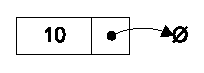
\includegraphics{singly_linked_list_node}
\end{center}
\caption{Singly linked list node}
\end{figure}

\subsection{Insertion} \label{single_insertion}
In general when people talk about insertion with respect to linked lists of any form they implicitly refer to the adding of a node to the tail of the list, thus when you use an API like that of DSA and you see a general purpose method that adds a node to the list assume that you are adding that node to the tail of the list not the head.

Adding a node to a singly linked list has only two cases: 
\begin{enumerate}
\item $head = \emptyset$ in which case the node we are adding is now both the $head$ and $tail$ of the list; or
\item we simply need to append our node onto the end of the list updating the $tail$ reference appropriately.
\end{enumerate}

\begin{tabbing}
1)  \textbf{alg}\= \textbf{orithm} Add($value$) \\
2)  \> \textbf{Pre:}~~$value$ is the value to add to the list \\
3)  \> \textbf{Post:}~$value$ has been placed at the tail of the list \\
4)  \> $n \leftarrow$ node($value$) \\
5)  \> \textbf{if}~\= $head = \emptyset$ \\
6)  \> \> $head \leftarrow n$ \\
7)  \> \> $tail \leftarrow n$ \\
8)  \> \textbf{else} \\
9)  \> \> $tail$.Next $\leftarrow n$ \\
10) \> \> $tail \leftarrow n$ \\
11) \> \textbf{end if} \\
12) \textbf{end} Add \\
\end{tabbing}

As an example of the previous algorithm consider adding the following sequence of integers to the list: $1$, $45$, $60$, and $12$, the resulting list is that of Figure \ref{fig:singly_populated_list}.

\begin{figure}
\begin{center}
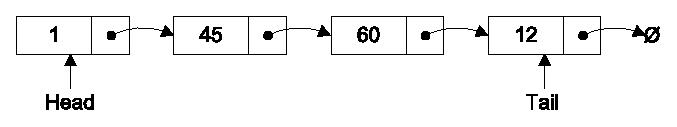
\includegraphics{singly_linked_list_populated_list}
\end{center}
\caption{A singly linked list populated with integers} \label{fig:singly_populated_list}
\end{figure}

\subsection{Searching} \label{single_search}
Searching a linked list is straight forward, we simply traverse the list checking the value we are looking for with the value of each node in the linked list. The algorithm listed in this section is very similar to that used for traversal in \S\ref{singly_linked_traversal}.

\begin{tabbing}
1)  \textbf{alg}\= \textbf{orithm} Contains($head$, $value$) \\
2)  \> \textbf{Pre:}~~$head$ is the head node in the list \\
3)  \> ~~~~~~~~$value$ is the value to search for \\
4)  \> \textbf{Post:}~the item is either in the linked list, true; otherwise false \\
5)  \> $n \leftarrow head$ \\
6)  \> \textbf{whi}\= \textbf{le} $n~!= \emptyset$ \textbf{and} $n$.Value $!= value$ \\
7)  \> \> $n \leftarrow n$.Next \\
8)  \> \textbf{end while} \\
9)  \> \textbf{if} $n = \emptyset$ \\
10) \> \> \textbf{return false} \\
11) \> \textbf{else} \\
12) \> \> \textbf{return true} \\
13) \> \textbf{end if} \\
14) \textbf{end} Contains \\
\end{tabbing}

\subsection{Deletion} \label{single_deletion}
Deleting a node from a linked list is straight forward but there are a few cases in which we need to accommodate for:
\begin{enumerate}
\item the list is empty; or
\item the node to remove is the only node in the linked list; or 
\item we are removing the head node; or
\item we are removing the tail node; or
\item the node to remove is somewhere in between the head and tail; or
\item the item to remove doesn't exist in the linked list
\end{enumerate}

The algorithm whose cases we have described will remove a node from anywhere within a list irrespective of whether the node is the $head$ etc. If at all possible you know that items will only ever be removed from the $head$ or $tail$ of the list then you can create much more concise algorithms, in the case of always removing  from the front of the linked list deletion becomes an $O(1)$ operation.

\newpage
\begin{tabbing}
1)  \textbf{alg}\= \textbf{orithm} Remove($head$, $value$) \\
2)  \> \textbf{Pre:}~~$head$ is the head node in the list \\
3)  \> ~~~~~~~~$value$ is the value to remove from the list \\
4)  \> \textbf{Post:}~$value$ is removed from the list, true; otherwise false \\
5)  \> \textbf{if}~\= $head = \emptyset$ \\
6)  \> \> // case 1 \\
7)  \> \> \textbf{return false} \\
8)  \> \textbf{end if} \\
9)  \> $n \leftarrow head$ \\
10) \> \textbf{if} $n$.Value $= value$ \\
11) \> \> \textbf{if}~\= $n = head$ \textbf{and} $n = tail$ \\
12) \> \> \> // case 2 \\
13) \> \> \> $head \leftarrow \emptyset$ \\
14) \> \> \> $tail \leftarrow \emptyset$ \\
15) \> \> \textbf{else} \\
16) \> \> \> // case 3 \\
17) \> \> \> $head \leftarrow head$.Next \\
18) \> \> \textbf{end if} \\
19) \> \> \textbf{return true} \\
20) \> \textbf{end if} \\
21) \> \textbf{while} $n$.Next $!= \emptyset$ \textbf{and} $n$.Next.Value $!= value$ \\
22) \> \> $n \leftarrow n$.Next \\
23) \> \textbf{end while} \\
24) \> \textbf{if} $n$.Next $!= \emptyset$ \textbf{and} $n$.Next.Value $= value$ \\
25) \> \> \textbf{if} $n$.Next $= tail$ \\
26) \> \> \> // case 4 \\
27) \> \> \> $tail \leftarrow n$ \\
28) \> \> \textbf{end if} \\
29) \> \> // this is only case 5 if the conditional on line 25) was $ff$ \\
30) \> \> $n$.Next $\leftarrow n$.Next.Next \\
31) \> \> \textbf{return true} \\
32) \> \textbf{end if} \\
33) \> // case 6 \\
34) \> \textbf{return false} \\
35) \textbf{end} Remove \\
\end{tabbing}

\subsection{Traversing the list} \label{singly_linked_traversal}
Traversing a singly list is the same as that of traversing a doubly linked list (defined in \S\ref{doubly_linked_list}), you start at the head of the list and continue until you come across a node that is $\emptyset$. The two cases are as follows:

\begin{enumerate}
\item $node = \emptyset$, we have exhausted all nodes in the linked list; or
\item we must update the $node$ reference to be $node$.Next.
\end{enumerate}

The algorithm described is a very simple one that makes use of a simple $while$ loop to check the first case. 

\newpage
\begin{tabbing}
1)  \textbf{alg}\= \textbf{orithm} Traverse($head$) \\
2)  \> \textbf{Pre:}~~$head$ is the head node in the list \\
3)  \> \textbf{Post:}~the items in the list have been traversed \\
4)  \> $n \leftarrow head$ \\
5)  \> \textbf{whi}\=\textbf{le} $n~!= 0$ \\
6)  \> \> \textbf{yield} $n$.Value \\
7)  \> \> $n \leftarrow n$.Next \\
8)  \> \textbf{end while} \\
9)  \textbf{end} Traverse \\
\end{tabbing}

\subsection{Traversing the list in reverse order}
Traversing a singly linked list in a forward manned is simple (i.e. left to right) as demonstrated in \S\ref{singly_linked_traversal}, however, what if for some reason we wanted to traverse the nodes in the linked list in reverse order? The algorithm to perform such a traversal is very simple, and just like demonstrated in \S\ref{single_deletion} we will need to acquire a reference to the previous node of a node, even though the fundamental characteristics of the nodes that make up a singly linked list prohibit this by design.

The following algorithm being applied to a linked list with the integers $5$, $10$, $1$, and $40$ is depicted in Figure \ref{fig:singly_linked_list_reverse_traversal}.

\begin{tabbing}
1)  \textbf{alg}\= \textbf{orithm} ReverseTraversal($tail$) \\
2)  \> \textbf{Pre:}~~$tail$ is the tail node in the list \\
3)  \> \textbf{Post:}~the items in the list have been traversed in reverse order \\
4)  \> \textbf{if}~\= $tail~!= \emptyset$ \\
5)  \> \> $curr \leftarrow tail$ \\
6)  \> \> \textbf{whi}\= \textbf{le} $curr~!= head$ \\
7)  \> \> \> $prev \leftarrow head$ \\
8)  \> \> \> \textbf{whi}\= \textbf{le} $prev$.Next $!= curr$ \\
9)  \> \> \> \> $prev \leftarrow prev$.Next \\
10) \> \> \> \textbf{end while} \\
11) \> \> \> \textbf{yield} $curr$.Value \\
12) \> \> \> $curr \leftarrow prev$ \\
13) \> \> \textbf{end while} \\
14) \> \> \textbf{yield} $curr$.Value \\
15) \> \textbf{end if} \\
16) \textbf{end} ReverseTraversal \\
\end{tabbing}

This algorithm is only of real interest when we are using singly linked lists, as you will soon find out doubly linked lists (defined in \S\ref{doubly_linked_list}) have certain properties that remove the challenge of reverse list traversal.

\begin{figure}
\begin{center}
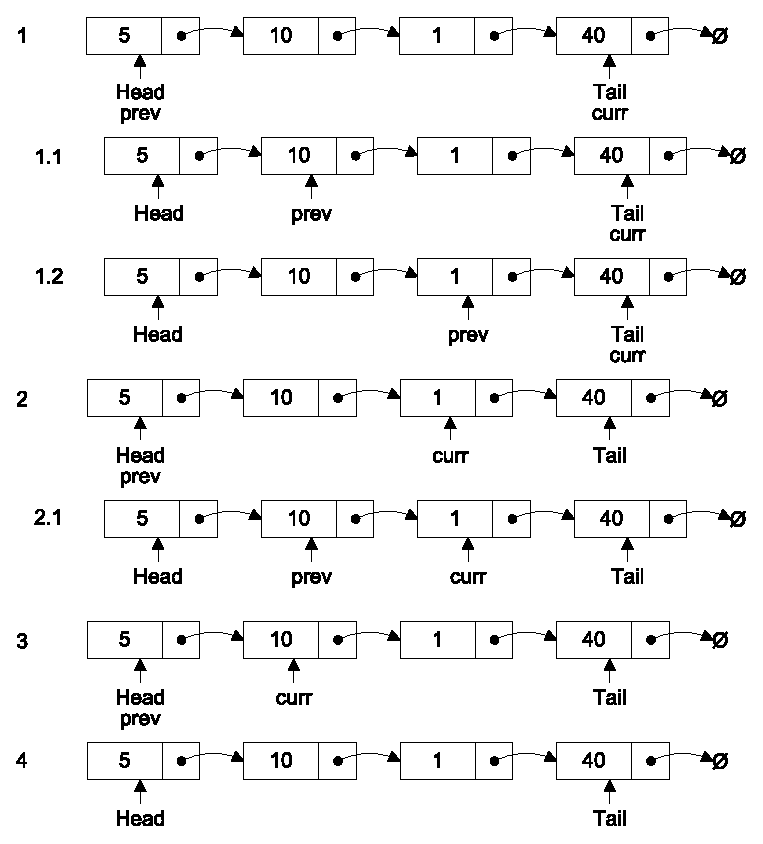
\includegraphics{singly_linked_list_reverse_traversal}
\end{center}
\caption{Reverse traveral of a singly linked list} \label{fig:singly_linked_list_reverse_traversal}
\end{figure}

\section{Doubly Linked List} \label{doubly_linked_list}
Doubly linked lists are very similar to singly linked lists, the only difference is that each node has a reference to both the next and previous nodes in the list.

\begin{figure}
\begin{center}
\includegraphics{doubly_linked_list_node}
\end{center}
\caption{Doubly linked list node}
\end{figure}


It would be wise to point out that the following algorithms for the doubly linked list are exactly the same as those listed previously for the singly linked list:

\begin{enumerate}
\item Searching (defined in \S\ref{single_search})
\item Traversal (defined in \S\ref{singly_linked_traversal})
\end{enumerate}

\subsection{Insertion}
The only major difference between the algorithm in \S\ref{single_insertion} is that we need to remember to bind the previous pointer of $n$ to the previous tail node if $n$ was not the first node to be inserted into the list.

\begin{tabbing}
1)  \textbf{alg}\= \textbf{orithm} Add($value$) \\
2)  \> \textbf{Pre:}~~$value$ is the value to add to the list \\
3)  \> \textbf{Post:}~$value$ has been placed at the tail of the list \\
4)  \> $n \leftarrow$ node($value$) \\
5)  \> \textbf{if}~\= $head = \emptyset$ \\
6)  \> \> $head \leftarrow n$ \\
7)  \> \> $tail \leftarrow n$ \\
8)  \> \textbf{else} \\
9)  \> \> $n$.Previous $\leftarrow tail$ \\
10) \> \> $tail$.Next $\leftarrow n$ \\
11) \> \> $tail \leftarrow n$ \\
12) \> \textbf{end if} \\
13) \textbf{end} Add \\
\end{tabbing}

Figure \ref{fig:doubly_linked_list_add} shows the doubly linked list after adding the sequence of integers defined in \S\ref{single_insertion}.

\begin{figure}[h]
\begin{center}
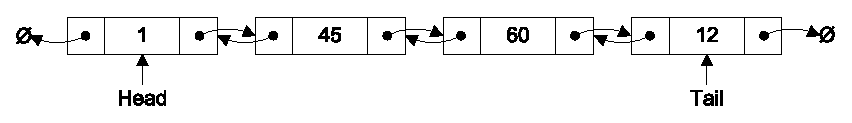
\includegraphics{doubly_linked_list_populated}
\end{center}
\caption{Doubly linked list populated with integers} \label{fig:doubly_linked_list_add}
\end{figure}

\subsection{Deletion}
As you may of guessed the cases that we use for deletion in a doubly linked list are exactly the same as those defined in \S\ref{single_deletion}, however, like insertion we have the added task of binding an additional reference ($Previous$) to the correct value.

\newpage
\begin{tabbing}
1)  \textbf{alg}\= \textbf{orithm} Remove($head$, $value$) \\
2)  \> \textbf{Pre:}~~$head$ is the head node in the list \\
3)  \> ~~~~~~~~$value$ is the value to remove from the list \\
4)  \> \textbf{Post:}~$value$ is removed from the list, true; otherwise false \\
5)  \> \textbf{if}~\= $head = \emptyset$ \\
6)  \> \> \textbf{return false} \\
7)  \> \textbf{end if} \\
8)  \> \textbf{if} $value = head$.Value \\
9)  \> \> \textbf{if}~\= $head = tail$ \\
10) \> \> \> $head \leftarrow \emptyset$ \\
11) \> \> \> $tail \leftarrow \emptyset$ \\
12) \> \> \textbf{else} \\
13) \> \> \> $head \leftarrow head$.Next \\
14) \> \> \> $head$.Previous $\leftarrow \emptyset$ \\
15) \> \> \textbf{end if} \\
16) \> \> \textbf{return true} \\
17) \> \textbf{end if} \\
18) \> $n \leftarrow head$.Next \\
19) \> \textbf{while} $n~!= \emptyset$ \textbf{and} $value~!= n$.Value \\
20) \> \> $n \leftarrow n$.Next \\
21) \> \textbf{end while} \\
22) \> \textbf{if} $n = tail$ \\
23) \> \> $tail \leftarrow tail$.Previous \\
24) \> \> $tail$.Next $\leftarrow \emptyset$ \\
25) \> \> \textbf{return true} \\
26) \> \textbf{else if} $n~!= \emptyset$ \\
27) \> \> $n$.Previous.Next $\leftarrow n$.Next \\
28) \> \> $n$.Next.Previous $\leftarrow n$.Previous \\
29) \> \> \textbf{return true} \\
30) \> \textbf{end if} \\
31) \> \textbf{return false} \\
32) \textbf{end} Remove \\
\end{tabbing}

% Copyright (C) Data Structures and Algorithms Team.
\chapter{Binary Search Tree} \label{bst}
Binary search tree's (BSTs) are very simple to understand, consider the following where by we have a root node $n$, the left sub tree of $n$ contains values $< n$, the right sub tree however contains nodes whose values are $\geq n$.

BSTs are of interest because they have operations which are favourably fast, insertion, look up, and deletion can all be done in $O(log~n)$. One of the things that I would like to point out and address early is that $O(log~n)$ times for the aforementioned operations can only be attained if the BST is relatively balanced (for a tree data structure with self balancing properties see \S\ref{Avl}). 

\begin{figure}[htp]
\begin{center}
\includegraphics{bst_intro}
\end{center}
\caption{Simple unbalanced binary search tree} \label{fig:bst_intro}
\end{figure}

\newpage
\section{Insertion}
As mentioned previously insertion is an $O(log~n)$ operation provided that the tree is moderately balanced.

\begin{tabbing}
1)  \textbf{alg}\= \textbf{orithm} Insert($value$) \\
2)  \> \textbf{Pre:}~~$value$ has passed custom type checks for type $T$ \\
3)  \> \textbf{Post:}~$value$ has been placed in the correct location in the tree \\
4)  \> \textbf{if}~\= $root~= \emptyset$ \\
5)  \> \> $root \leftarrow$ node($value$) \\
6)  \> \textbf{else} \\
7)  \> \> InsertNode($root$, $value$) \\
8)  \> \textbf{end if} \\
9)  \textbf{end} Insert \\
\end{tabbing}


\begin{tabbing}
1)  \textbf{alg}\= \textbf{orithm} InsertNode($root$, $value$) \\
2)  \> \textbf{Pre:}~~$root$ is the node to start from \\
3)  \> \textbf{Post:}~$value$ has been placed in the correct location in the tree \\
4)  \> \textbf{if}~\= $value < root$.Value \\
5)  \> \> \textbf{if}~\= $root$.Left $= \emptyset$ \\
6)  \> \> \> $root$.Left $\leftarrow$ node($value$) \\
7)  \> \> \textbf{else} \\
8)  \> \> \> InsertNode($root$.Left, $value$) \\
9)  \> \> \textbf{end if} \\
10) \> \textbf{else} \\
11) \> \> \textbf{if} $root$.Right $= \emptyset$ \\
12) \> \> \> $root$.Right $\leftarrow$ node($value$) \\
13) \> \> \textbf{else} \\
14) \> \> \> InsertNode($root$.Right, $value$) \\
15) \> \> \textbf{end if} \\
16) \> \textbf{end if} \\
17) \textbf{end} InsertNode \\ 
\end{tabbing}

The insertion algorithm is split for a good reason, the first algorithm (non-recursive) checks a very core base case - whether or not the tree is empty, if the tree is empty then we simply create our root node and we have no need to invoke the recursive $InsertNode$ algorithm. When the core base case is not met we must invoke the recursive $InsertNode$ algorithm which simply guides us to the first appropriate place in the tree to put $value$.

\newpage
\section{Searching}
Searching a BST is really quite simple, the pseudo code is self explanatory but I will explain briefly the premise of the algorithm nonetheless.

We have talked previously about insertion, we go either left or right with the right sub tree containing values that are $\geq n$ where $n$ is the value of the node we are inserting, when searching the rules are made a little more atomic and at any one time we have four cases to consider: 
\begin{enumerate}
\item the $root = \emptyset$ in which case $value$ is not in the BST; or
\item $root$.Value $= value$ in which case $value$ is in the BST; or
\item $value < root$.Value, we must inspect the left sub tree of $root$ for $value$; or
\item $value > root$.Value, we must inspect the right sub tree of $root$ for $value$.
\end{enumerate}



\begin{tabbing}
1)  \textbf{alg}\= \textbf{orithm} Contains($root$, $value$) \\
2)  \> \textbf{Pre:}~~$root$ is the root node of the tree, $value$ is what we would like to locate \\
3)  \> \textbf{Post:}~$value$ is either located or not \\
4)  \> \textbf{if}~\= $root = \emptyset$ \\
5)  \> \> \textbf{return false} \\
6)  \> \textbf{end if} \\
7)  \> \textbf{if} $root$.Value $= value$ \\
8)  \> \> \textbf{return true} \\
9)  \> \textbf{else if} $value < root$.Value \\
10) \> \> \textbf{return} Contains($root$.Left, $value$) \\
11) \> \textbf{else} \\
12) \> \> \textbf{return} Contains($root$.Right, $value$) \\
13) \> \textbf{end if} \\
14) \textbf{end} Contains \\
\end{tabbing}

\newpage
\section{Deletion}
Removing a node from a BST is simple, there are four cases that we must consider though: 
\begin{enumerate}
\item the value to remove is a leaf node; or
\item the value to remove has a right sub tree, but no left sub tree; or
\item the value to remove has a left sub tree, but no right sub tree; or
\item the value to remove has both a left and right sub tree in which case we promote the largest value in the left sub tree.
\end{enumerate}
\begin{figure}[htp]
\begin{center}
\includegraphics{bst_deletion}
\end{center}
\caption{binary search tree deletion cases} \label{fig:bst_deletion}
\end{figure}

The $Remove$ algorithm described later relies on two further helper algorithms named $FindParent$, and $FindNode$ which are described in \S\ref{finding_parent_node} and \S\ref{find_node_reference}.

\newpage
\begin{tabbing}
1)  \textbf{alg}\= \textbf{orithm} Remove($value$) \\
2)  \> \textbf{Pre:}~~$value$ is the value of the node to remove, $root$ is the root node of the BST \\
3)  \> \textbf{Post:}~node with $value$ is removed if found in which case yields true, otherwise false \\
4)  \> $nodeToRemove \leftarrow$ FindNode($value$) \\
5)  \> \textbf{if}~\= $nodeToRemove = \emptyset$ \\
6)  \> \> \textbf{return false} // value not in BST \\
7)  \> \textbf{end if} \\
8)  \> $parent \leftarrow$ FindParent($value$) \\
9)  \> \textbf{if} $count = 1$ // $count$ keeps track of the \# of nodes in the BST \\
10) \> \> $root \leftarrow \emptyset$ // we are removing the only node in the BST \\
11) \> \textbf{else if} $nodeToRemove$.Left $= \emptyset$ \textbf{and} $nodeToRemove$.Right $= null$ \\
12) \> \> // case \#1 \\
13) \> \> \textbf{if}~\= $nodeToRemove$.Value $< parent$.Value \\
14) \> \> \> $parent$.Left $\leftarrow \emptyset$ \\
15) \> \> \textbf{else} \\
16) \> \> \> $parent$.Right $\leftarrow \emptyset$ \\
17) \> \> \textbf{end if} \\
18) \> \textbf{else if} $nodeToRemove$.Left $= \emptyset$ \textbf{and} $nodeToRemove$.Right $!= \emptyset$ \\
19) \> \> // case \# 2 \\
20) \> \> \textbf{if} $nodeToRemove$.Value $< parent$.Value \\
21) \> \> \> $parent$.Left $\leftarrow nodeToRemove$.Right \\
22) \> \> \textbf{else} \\
23) \> \> \> $parent$.Right $\leftarrow nodeToRemove$.Right \\
24) \> \> \textbf{end if} \\
25) \> \textbf{else if} $nodeToRemove$.Left $!= \emptyset$ \textbf{and} $nodeToRemove$.Right $= \emptyset$ \\
26) \> \> // case \#3 \\
27) \> \> \textbf{if} $nodeToRemove$.Value $< parent$.Value \\
28) \> \> \> $parent$.Left $\leftarrow nodeToRemove$.Left \\
29) \> \> \textbf{else} \\
30) \> \> \> $parent$.Right $\leftarrow nodeToRemove$.Left \\
31) \> \> \textbf{end if} \\
32) \> \textbf{else} \\
33) \> \> // case \#4 \\
34) \> \> $largestValue \leftarrow nodeToRemove$.Left \\
35) \> \> \textbf{while} $largestValue$.Right $!= \emptyset$ \\
36) \> \> \> // find the largest value in the left sub tree of $nodeToRemove$ \\
37) \> \> \> $largestValue \leftarrow largestValue$.Right \\
38) \> \> \textbf{end while} \\
39) \> \> // set the parents' Right pointer of $largestValue$ to $\emptyset$ \\
40) \> \> FindParent($largestValue$.Value).Right $\leftarrow \emptyset$ \\
41) \> \> $nodeToRemove$.Value $\leftarrow largestValue$.Value \\
42) \> \textbf{end if} \\
43) \> $count \leftarrow count - 1$ \\
44) \> \textbf{return true} \\
45) \textbf{end} Remove \\
\end{tabbing}

\section{Finding the parent of a given node} \label{finding_parent_node}
The purpose of this algorithm is simple - to return a reference (or a pointer) to the parent node of the node with the given value. We have found that such an algorithm is very useful, especially when performing extensive tree transformations.

\begin{tabbing}
1)  \textbf{alg}\= \textbf{orithm} FindParent($value$, $root$) \\
2)  \> \textbf{Pre:}~~$value$ is the value of the node we want to find the parent of \\
3)  \> ~~~~~~~~$root$ is the root node of the BST and is $!= \emptyset$ \\
4)  \> \textbf{Post:}~a reference to the parent node of $value$ if found; otherwise $\emptyset$ \\
5)  \> \textbf{if}~\= $value = root$.Value \\
6)  \> \> \textbf{return} $\emptyset$ \\
7)  \> \textbf{end if} \\
8)  \> \textbf{if} $value < root$.Value \\
9)  \> \> \textbf{if}~\= $root$.Left $= \emptyset$ \\
10) \> \> \> \textbf{return} $\emptyset$ \\
11) \> \> \textbf{else if} $root$.Left.Value $= value$ \\
12) \> \> \> \textbf{return} $root$ \\
13) \> \> \textbf{else} \\
14) \> \> \> \textbf{return} FindParent($value$, $root$.Left) \\
15) \> \> \textbf{end if} \\
16) \> \textbf{else} \\
17) \> \> \textbf{if} $root$.Right $= \emptyset$ \\
18) \> \> \> \textbf{return} $\emptyset$ \\
19) \> \> \textbf{else if} $root$.Right.Value $= value$ \\
20) \> \> \> \textbf{return} $root$ \\
21) \> \> \textbf{else} \\
22) \> \> \> \textbf{return} FindParent($value$, $root$.Right) \\
23) \> \> \textbf{end if} \\
24) \> \textbf{end if} \\
25) \textbf{end} FindParent \\
\end{tabbing}

\section{Attaining a reference to a node} \label{find_node_reference}
Just like the algorithm explained in \S\ref{finding_parent_node} this algorithm we have found to be very useful, it simply finds the node with the specified value and returns a reference to that node.

\newpage
\begin{tabbing}
1)  \textbf{alg}\= \textbf{orithm} FindNode($value$, $root$) \\
2)  \> \textbf{Pre:}~~$value$ is the value of the node we want to find the parent of \\
3)  \> ~~~~~~~~$root$ is the root node of the BST \\
4)  \> \textbf{Post:}~a reference to the node of $value$ if found; otherwise $\emptyset$ \\
5)  \> \textbf{if}~\= $root = \emptyset$ \\
6)  \> \> \textbf{return} $\emptyset$ \\
7)  \> \textbf{end if} \\
8)  \> \textbf{if} $value < root$.Value \\
9)  \> \> \textbf{return} FindNode($value$, $root$.Left) \\
10) \> \textbf{else if} $value > root$.Value \\
11) \> \> \textbf{return} FindNode($value$, $root$.Right) \\
12) \> \textbf{else} \\
13) \> \> \textbf{return} $root$ \\
14) \> \textbf{end if} \\
15) \textbf{end} FindNode \\
\end{tabbing}

\section{Finding the smallest and largest values in the binary search tree}
A simple task, to find the smallest value in a BST you simply traverse the nodes in the left sub tree of the BST always going left upon each encounter with a node, the opposite is the case when finding the largest value in the BST. Both algorithms are incredibly simple, they are listed simply for completeness.

The base case in both $FindMin$, and $FindMax$ algorithms is when the Left ($FindMin$), or Right ($FindMax$) node references are $\emptyset$.

\begin{tabbing}
1)  \textbf{alg}\= \textbf{orithm} FindMin($root$) \\
2)  \> \textbf{Pre:}~~$root$ is the root node of the BST \\
3)  \> ~~~~~~~~$root$ $!= \emptyset$ \\
4)  \> \textbf{Post:}~the smallest value in the BST is located \\
5)  \> \textbf{if}~\= $root$.Left $= \emptyset$ \\
6)  \> \> \textbf{return} $root$.Value \\
7)  \> \textbf{end if} \\
8)  \> FindMin($root$.Left) \\
9)  \textbf{end} FindMin \\
\end{tabbing}

\begin{tabbing}
1)  \textbf{alg}\= \textbf{orithm} FindMax($root$) \\
2)  \> \textbf{Pre:}~~$root$ is the root node of the BST \\
3)  \> ~~~~~~~~$root$ $!= \emptyset$ \\
4)  \> \textbf{Post:}~the largest value in the BST is located \\
5)  \> \textbf{if}~\= $root$.Right $= \emptyset$ \\
6)  \> \> \textbf{return} $root$.Value \\
7)  \> \textbf{end if} \\
8)  \> FindMax($root$.Right) \\
9)  \textbf{end} FindMax \\
\end{tabbing}

\section{Tree Traversals}
For the most part when you have a tree you will want to traverse the items in that tree using various strategies in order to attain the node visitation order you require. In this section we will touch on the traversals that DSA provides on all data structures that derive from $BinarySearchTree$.

\subsection{Preorder} \label{preorder_traversal}
When using the preorder algorithm, you visit the root first, traverse the left sub tree and traverse the right sub tree. An example of preorder traversal is shown in Figure \ref{fig:bst_preorder}.
\begin{figure}[htp]
\begin{center}
\includegraphics{bst_preorder}
\end{center}
\caption{Preorder visit binary search tree example} \label{fig:bst_preorder}
\end{figure}


\begin{tabbing}
1)  \textbf{alg}\= \textbf{orithm} Preorder($root$) \\
2)  \> \textbf{Pre:}~~$root$ is the root node of the BST \\
3)  \> \textbf{Post:}~the nodes in the BST have been visited in preorder \\
4)  \> \textbf{if}~\= $root~!= \emptyset$ \\
5)  \> \> \textbf{yield} $root$.Value \\
6)  \> \> Preorder($root$.Left) \\
7)  \> \> Preorder($root$.Right) \\
8)  \> \textbf{end if} \\
9)  \textbf{end} Preorder \\
\end{tabbing}

\subsection{Postorder} \label{postorder_traversal}
This algorithm is very similar to that described in \S\ref{preorder_traversal}, however the value of the node is yielded after traversing the left sub tree and  the right sub tree. An example of postorder traversal is shown in figure \ref{fig:bst_postorder}.

\begin{figure}[htp]
\begin{center}
\includegraphics{bst_postorder}
\end{center}
\caption{Postorder visit binary search tree example} \label{fig:bst_postorder}
\end{figure}

\begin{tabbing}
1)  \textbf{alg}\= \textbf{orithm} Postorder($root$) \\
2)  \> \textbf{Pre:}~~$root$ is the root node of the BST \\
3)  \> \textbf{Post:}~the nodes in the BST have been visited in postorder \\
4)  \> \textbf{if}~\= $root~!= \emptyset$ \\
5)  \> \> Postorder($root$.Left) \\
6)  \> \> Postorder($root$.Right) \\
7)  \> \> \textbf{yield} $root$.Value \\
8)  \> \textbf{end if} \\
9)  \textbf{end} Postorder \\
\end{tabbing}

\newpage
\subsection{Inorder}
Another variation of the algorithms defined in \S\ref{preorder_traversal} and \S\ref{postorder_traversal} is that of inorder traversal where the value of the current node is yielded in between traversing the left sub tree and  the right sub tree. An example of inorder traversal is shown in Figure \ref{fig:bst_inorder}.

\begin{figure}[htp]
\begin{center}
\includegraphics{bst_inorder}
\end{center}
\caption{Inorder visit binary search tree example} \label{fig:bst_inorder}
\end{figure}


\begin{tabbing}
1)  \textbf{alg}\= \textbf{orithm} Inorder($root$) \\
2)  \> \textbf{Pre:}~~$root$ is the root node of the BST \\
3)  \> \textbf{Post:}~the nodes in the BST have been visited in inorder \\
4)  \> \textbf{if}~\= $root~!= \emptyset$ \\
5)  \> \> Inorder($root$.Left) \\
6)  \> \> \textbf{yield} $root$.Value \\
7)  \> \> Inorder($root$.Right) \\
8)  \> \textbf{end if} \\
9)  \textbf{end} Inorder \\
\end{tabbing}

\subsection{Breadth First} \label{breadth_first}
Traversing a tree in breadth first order is to yield the values of all nodes of a particular depth in the tree, e.g. given the depth $d$ we would visit the values of all nodes in a left to right fashion at $d$, then we would proceed to $d+1$ and so on until we had ran out of nodes to visit. An example of breadth first traversal is shown in Figure \ref{fig:bst_breadth}.

Traditionally the way breadth first is implemented is using a list (vector, resizeable array, etc) to store the values of the nodes visited in breadth first order and then a queue to store those nodes that have yet to be visited.

\begin{figure}[htp]
\begin{center}
\includegraphics{bst_breadth}
\end{center}
\caption{Breadth First visit binary search tree example} \label{fig:bst_breadth}
\end{figure}

\newpage
\begin{tabbing}
1)  \textbf{alg}\= \textbf{orithm} BreadthFirst($root$) \\
2)  \> \textbf{Pre:}~~$root$ is the root node of the BST \\
3)  \> \textbf{Post:}~the nodes in the BST have been visited in breadth first order \\
4)  \> $l \leftarrow$ list \\
5)  \> $q \leftarrow$ queue \\
6)  \> \textbf{whi}\= \textbf{le} $root~!= \emptyset$ \\
7)  \> \> $l$.Add($root$.Value) \\
8)  \> \> \textbf{if}~\= $root$.Left $!= \emptyset$ \\
9)  \> \> \> $q$.Enqueue($root$.Left) \\
10) \> \> \textbf{end if} \\
11) \> \> \textbf{if} $root$.Right $!= \emptyset$ \\
12) \> \> \> $q$.Enqueue($root$.Right) \\
13) \> \> \textbf{end if} \\
14) \> \> \textbf{if} $!q$.IsEmpty() \\
15) \> \> \> $root \leftarrow q$.Dequeue() \\
16) \> \> \textbf{else} \\
17) \> \> \> $root \leftarrow \emptyset$ \\
18) \> \> \textbf{end if} \\
19) \> \textbf{end while} \\
20) \> \textbf{return} $l$ \\
21) \textbf{end} BreadthFirst \\
\end{tabbing}

% Copyright (C) Data Structures and Algorithms Team.
\chapter{Heap}
A heap can be thought of as a simple tree data structure, however a heap usually employs one of two strategies:

\begin{enumerate}
\item min heap; or
\item max heap
\end{enumerate}

Each strategy determines the properties of the tree and it's values, e.g. if you were to choose the strategy min heap then each parent node would have a value that is $\leq$ than it's children, thus the node at the root of the tree will have the smallest value in the tree, the opposite is true if you were to use max heap. Generally as a rule you should always assume that a heap employs the min heap strategy unless otherwise stated.

Unlike other tree data structures like the one defined in \S\ref{bst} a heap is generally implemented as an array rather than a series of nodes who each have references to other nodes, both however contain nodes that have at most two children. Figure \ref{fig:tree_array_representation} shows how the tree (not a heap data structure) ($12~7$($3~2$)~$6$($9$~~)) would be represented as an array.

\begin{figure}
\begin{center}
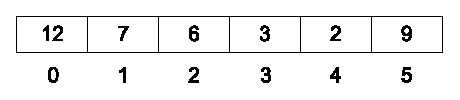
\includegraphics{heap_tree_array_representation}
\end{center}
\caption{Array representation of a simple tree data structure} \label{fig:tree_array_representation}
\end{figure}

Because we are using an array we need some way to calculate the index of a parent node, and the children of a node this is very simple, the expressions are defined below:

\begin{enumerate}
\item ($index - 1$)/$2$ (parent index)
\item $2 * index + 1$ (left child)
\item $2 * index + 2$ (right child)
\end{enumerate}

In Figure \ref{fig:heap_tree_array_representation_indexes} a) represents the calculation of the right child of $12$ ($2 * 0 + 2$); and b) calculates the index of the parent of $3$ (($3 - 1$)/$2$).

\begin{figure}
\begin{center}
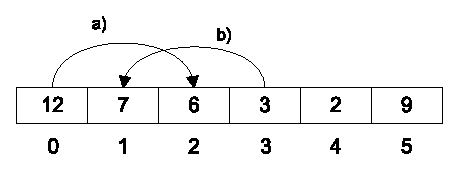
\includegraphics{heap_tree_array_representation_indexes}
\caption{Calculating node properties} \label{fig:heap_tree_array_representation_indexes}
\end{center}
\end{figure}

\section{Insertion}
Adding an item to a heap has an $O(log~n)$ run time complexity, this is due to the fact that after every insertion we must verify that the heap ordering strategy used is preserved, if not we must swap the values appropriately as we work up through the sub tree's starting with the sub tree the last value was added to.


Designing an algorithm for heap insertion is simple, however we must ensure that heap order is preserved after each insertion - generally this is a post insertion operation. Inserting a value into the next free slot in an array is simple, we just need to keep track of, and increment a counter after each insertion that tells us the next free index in the array. Inserting our value into the heap is the first part of the algorithm, the second is validating heap order which in the case of min heap ordering requires us to swap the values of a parent and it's child if the value of the child is $<$ the value of it's parent, we must do this for each sub tree the value we just inserted is a constituent of.

Figure \ref{fig:heap_insertion_minify_steps} shows the steps of inserting the values $3$, $9$, $12$, $7$, and $1$ into a min heap.

\begin{figure}
\begin{center}
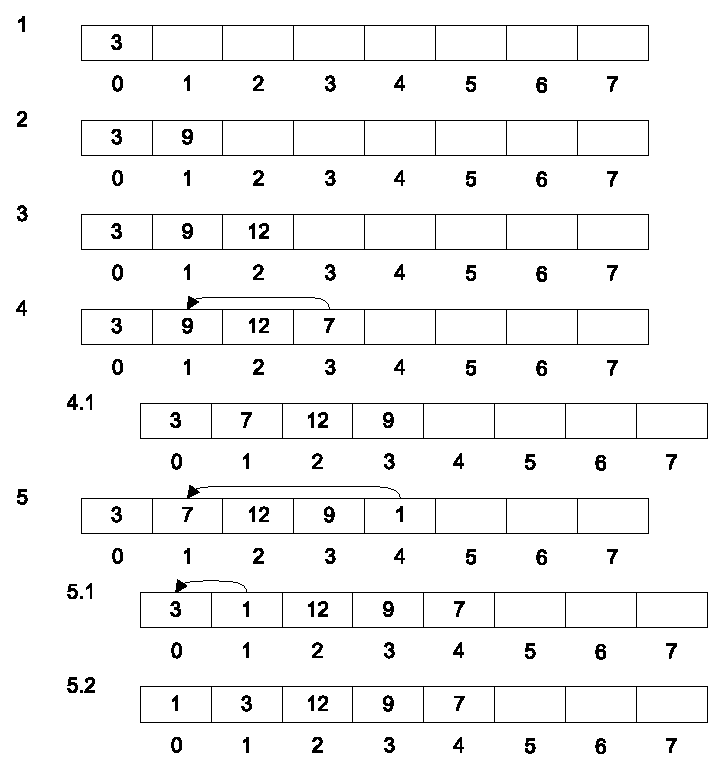
\includegraphics{heap_insertion_minify_steps}
\end{center}
\caption{Inserting values into a min heap} \label{fig:heap_insertion_minify_steps}
\end{figure}

\begin{tabbing}
1)  \textbf{alg}\= \textbf{orithm} Add($value$) \\
2)  \> \textbf{Pre:}~~$value$ is the value to add to the heap \\
3)  \> ~~~~~~~~Count is the number of items in the heap \\
4)  \> \textbf{Post:}~the value has been added to the heap \\
5)  \> $heap$[Count] $\leftarrow value$ \\
6)  \> Count $\leftarrow$ Count $+ 1$ \\
7)  \> MinHeapify() \\
8)  \textbf{end} Add \\
\end{tabbing}

\begin{tabbing}
1)  \textbf{alg}\= \textbf{orithm} MinHeapify() \\
2)  \> \textbf{Pre:}~~Count is the number of items in the heap \\
3)  \> ~~~~~~~~$heap$ is the array used to store the heap items \\
4)  \> \textbf{Post:}~the heap has preserved min heap ordering \\
5)  \> $i \leftarrow$ Count $- 1$ \\
6)  \> \textbf{whi}\= \textbf{le} $i >0$ \textbf{and} $heap$[$i$] $< heap$[($i - 1$)/$2$] \\
7)  \> \> Swap($heap$[$i$], $heap$[($i - 1$)/$2$] \\
8)  \> \> $i \leftarrow$ ($i - 1$)/$2$ \\
9)  \> \textbf{end while} \\
10) \textbf{end} MinHeapify \\
\end{tabbing}

% Copyright (C) Data Structures and Algorithms Team.
\chapter{Sets}
A set contains a number of values, the values are in no particular order and the values within the set are distinct from one another.

Generally set implementations tend to check that a value is not in the set first, before adding it to the set and so the issue of repeated values within the set is not an issue.

This section does not cover set theory in depth, rather it demonstrates briefly the ways in which the values of sets can be defined, and common operations that may be performed upon them.

The following $A = \{4, 7, 9, 12, 0\}$ defines a set $A$ whose values are listed within the curly braces. 

Given the set $A$ defined previously we can say that $4$ is a member of $A$ denoted by $4 \in A$, and that $99$ is not a member of $A$ denoted by $99 \notin A$.

Often defining a set by manually stating its members is tiresome, and more importantly the set may contain a large amount of values. A more concise way of defining a set and its members is by providing a series of properties that the values of the set must satisfy. In the following $A = \{x|x > 0, x~\%~2 = 0\}$ the set $A$ contains only positive integers that are even, $x$ is an alias to the current value we are inspecting and to the right hand side of $\mid$ are the properties that $x$ must satisfy to be in the set $A$ that is it must be $> 0$, and the remainder of the arithmetic expression $x / 2$ must be $0$.
You will be able to note from previous definition of the set $A$ that the set can contain an infinite number of values, and that the values of the set $A$ will be all even integers that are a member of the natural numbers set $\mathbb{N}$, where $\mathbb{N} = \{1, 2, 3, ...\}$.

Finally in this brief introduction to sets we will cover set intersection and union, both of which are very common operations (amongst many others) performed on sets. The union set can be defined as follows $A \cup B = \{x \mid x \in A~or~x \in B\}$, and intersection $A \cap B = \{x \mid x \in A~and~x \in B\}$. Figure \ref{fig:set_intersection_and_union} demonstrates set intersection and union graphically.

\begin{figure}
\begin{center}

\includegraphics{set_intersection_and_union}
\end{center}
\caption{a) $A \cap B$; b) $A \cup B$} \label{fig:set_intersection_and_union}
\end{figure} 

Given the following set definitions $A = \{1, 2, 3\}$, and $B = \{6, 2, 9\}$ the union of the two sets is $A \cup B= \{1, 2, 3, 6, 9\}$, and the intersection of the two sets is $A \cap B= \{2\}$.

Both set union and intersection are sometimes provided within the framework associated with mainstream languages, this is the case in .NET 3.5\footnote{\url{http://www.microsoft.com/NET/}} where such algorithms exist as extension methods defined in the type \textit{System.Linq.Enumerable}\footnote{\url{http://msdn.microsoft.com/en-us/library/system.linq.enumerable_members.aspx}}, as a result DSA does not provide implementations of these algorithms.

\section{Unordered}
Sets in the general sense do not enforce the explicit ordering of their members, for example the members of $B = \{6, 2, 9\}$ conform to no ordering scheme because it is not required. 

Most libraries provide implementations of unordered sets and so DSA does not, we simply mention it here to disambiguate between an unordered set and ordered set. 

We will only look at insertion for an unordered set and cover briefly why a hash table is an efficient data structure to use for its implementation.

\subsection{Insertion}
Unordered sets can be efficiently implemented using a hash table as its backing data structure. As mentioned previously we only add an item to a set if that item is not already in the set, thus the backing data structure we use must have a quick look up and insertion run time complexity.

A hash map generally provides the following:

\begin{enumerate}
\item $O(1)$ for insertion
\item approaching $O(1)$ for look up
\end{enumerate}

The above depends on how good the hashing algorithm of the hash table is, however most hash tables employ incredibly efficient general purpose hashing algorithms and so the run time complexities for the hash table in your library of choice should be very similar in terms of efficiency.

\section{Ordered}
An ordered set is similar to an unordered set in the sense that its members are distinct, however an ordered set enforces some predefined comparison on each of its members to result in a set whose members are ordered appropriately.

In DSA 0.5 and earlier we used a binary search tree (defined in \S\ref{bst}) as the internal backing data structure for our ordered set, from versions 0.6 onwards we replaced the binary search tree with an AVL tree primarily because AVL is balanced.

The ordered set has it's order realised by performing an inorder traversal upon its backing tree data structure which yields the correct ordered sequence of set members.

Because an ordered set in DSA is simply a wrapper for an AVL tree that additionally enforces the tree contains unique items you should read \S\ref{Avl} to learn more about the run time complexities associated with its operations.

% Copyright (C) Data Structures and Algorithms Team.
\chapter{Queues}
\section{Standard Queue}
\section{Priority Queue}

% Copyright (C) Data Structures and Algorithms Team.
\chapter{Balanced Trees} 
\section{AVL Tree} \label{Avl}


\part{Algorithms}
% Copyright (C) Data Structures and Algorithms Team.
\chapter{Sorting}
All the sorting algorithms in this chapter use data structures of a specific type to demonstrate sorting, e.g. a $32$ bit integer is often used as its associated operations (e.g. $<$, $>$, etc) are clear in their behaviour.

The algorithms discussed can easily be translated into generic sorting algorithms within your respective language of choice.
\newpage
\section{Bubble Sort}
One of the most simple forms of sorting is that of comparing each item with every other item in some list, however as the description may imply this form of sorting is not particularly effecient $O(n^{2})$. In it's most simple form bubble sort can be implemented as two loops.

\begin{figure}[h]
\begin{center}
\includegraphics{sorting_bubble}
\end{center}
\caption{Bubble Sort Iterations} \label{fig:sorting_bubble}
\end{figure}

\begin{tabbing}
1)  \textbf{alg}\= \textbf{orithm} BubbleSort($list$) \\
2)  \> \textbf{Pre:}~~$list~!= \emptyset$ \\
3)  \> \textbf{Post:}~$list$ has been sorted into values of ascending order \\
4)  \> \textbf{for}\=~$i \leftarrow 0$ to $list.Count - 1$ \\
5)  \> \> \textbf{for}\=~$j \leftarrow 0$ to $list.Count - 1$ \\
6)  \> \> \> \textbf{if}~\= $list[i] < list[j]$ \\
7)  \> \> \> \> $Swap(list[i], list[j])$ \\
8)  \> \> \> \textbf{end if} \\
9)  \> \> \textbf{end for} \\
10) \> \textbf{end for} \\
11) \> \textbf{return} $list$ \\
12) \textbf{end} BubbleSort
\end{tabbing}

\section{Merge Sort}
Merge sort is an algorithm that has a fairly effecient space time complexity - $O(n~log~n)$ and is fairly trivial to implement. The algorithm is based on splitting a list, into two similar sized lists ($left$, and $right$) and sorting each list and then merging the sorted lists back together. \textit{Note: the function MergeOrdered simply takes two ordered lists and makes them one.}

\begin{figure}[h]
\begin{center}
\includegraphics{sorting_merge}
\end{center}
\caption{Merge Sort Divide et Impera Approach} \label{fig:sorting_merge}
\end{figure}

\begin{tabbing}
1)  \textbf{alg}\= \textbf{orithm} Mergesort($list$) \\
2)  \> \textbf{Pre:}~~$list~!=~\emptyset$ \\
3)  \> \textbf{Post:}~$list$ has been sorted into values of ascending order \\
4)  \> \textbf{if}~\= $list$.Count $= 1$ // already sorted \\
5)  \> \> \textbf{return}~$list$ \\
6)  \> \textbf{end if} \\
7)  \> $m \leftarrow list$.Count $/~2$ \\
8)  \> $left \leftarrow$ list($m$) \\
9)  \> $right \leftarrow$ list($list$.Count $-~m$) \\
10) \> \textbf{for}\=~$i \leftarrow 0$ to $left$.Count$-1$ \\
11) \> \> $left$[$i$] $\leftarrow$ list[$i$] \\
12) \> \textbf{end for} \\
13) \> \textbf{for}\=~$i \leftarrow 0$ to $right$.Count$-1$ \\
14) \> \> $right$[$i$] $\leftarrow$ list[$i$] \\
15) \> \textbf{end for} \\
16) \> $left \leftarrow$ Mergesort($left$) \\
17) \> $right \leftarrow$ Mergesort($right$) \\
18) \> \textbf{return} MergeOrdered($left$, $right$) \\
19) \textbf{end} Mergesort \\
\end{tabbing}

\newpage
\section{Quick Sort} 
Quick sort is one of the most popular sorting algorithms based on divide et impera strategy, resulting in an $O(n~log~n)$ complexity. The algorithm starts by picking an item, called pivot, and moving all smaller items before it, while all greater elements after it. This is the main quick sort operation, called partition, recursively repeated on lesser and greater sub lists until their size  is one or zero - in which case the list is implicitly sorted.

Choosing an appropriate pivot, as for example the median element is fundamental for avoiding the drastically reduced performance of $O(n^{2})$.

\begin{tabbing}
1)  \textbf{alg}\= \textbf{orithm} QuickSort($list$) \\
2)  \> \textbf{Pre:}~~$list~!=~\emptyset$ \\
3)  \> \textbf{Post:}~$list$ has been sorted into values of ascending order \\
4)  \> \textbf{if}~\= $list$.Count $= 1$ // already sorted \\
5)  \> \> \textbf{return}~$list$ \\
6)  \> \textbf{end if} \\
7)  \> $pivot \leftarrow $MedianValue($list$) \\
8)  \> \textbf{for}\=~$i \leftarrow 0$ to $list$.Count$-1$ \\
9)  \> \> \textbf{if}~\= $list[i] = pivot$ \\
10) \> \> \> $equal$.Insert$(list[i])$\\
11) \> \> \textbf{end if} \\
12) \> \> \textbf{if}~\= $list[i] < pivot$ \\
13) \> \> \> $less$.Insert$(list[i])$\\
14) \> \> \textbf{end if} \\
15) \> \> \textbf{if}~\= $list[i] > pivot$ \\
16) \> \> \> $greater$.Insert$(list[i])$\\
17) \> \> \textbf{end if} \\
18) \> \textbf{end for} \\
19) \> \textbf{return} Concatenate(QuickSort($less$),~$equal$,~QuickSort($greater$)) \\
20) \textbf{end} Quicksort \\
\end{tabbing}

\newpage
\section{Insertion Sort} \label{shell_sort}
Insertion sort is a somewhat interesting algorithm with an expensive runtime of $O(n^{2})$. It can be best thought of as a sorting scheme similar to that of sorting a hand of playing cards, i.e. you take one card and then look at the rest with the intent of building up an ordered set of cards in your hand.

\begin{tabbing}
1)  \textbf{alg}\= \textbf{orithm} Insertionsort($list$) \\
2)  \> \textbf{Pre:}~~ $list~!=~\emptyset$ \\
3)  \> \textbf{Post:}~$list$ has been sorted into values of ascending order \\
4)  \> $unsorted \leftarrow 1$ \\
5)  \> \textbf{whi}\= \textbf{le} $unsorted < list$.Count \\
6)  \> \> $hold \leftarrow list$[$unsorted$] \\
7)  \> \> $i \leftarrow unsorted - 1$ \\
8)  \> \> \textbf{whi}\= \textbf{le} $i \geq 0$ \textbf{and} $hold < list$[$i$] \\
9)  \> \> \> $list$[$i + 1$] $\leftarrow$ $list$[$i$] \\
10) \> \> \> $i \leftarrow i - 1$ \\
11) \> \> \textbf{end while} \\
12) \> \> $list$[$i+1$] $\leftarrow hold$ \\
13) \> \> $unsorted \leftarrow unsorted + 1$ \\
14) \> \textbf{end while} \\
15) \> \textbf{return} $list$ \\
16) \textbf{end} Insertionsort \\
\end{tabbing}

\newpage
\section{Shell Sort}
Put simply shell sort can be thought of as a more efficient variation of insertion sort as described in \S\ref{shell_sort}, it achieves this mainly by comparing items of varying distances apart resulting in a run time complexity of $O(n~log^{2}~n)$.

Shell sort is fairly straight forward but may seem somewhat confusing at first as it differs from other sorting algorithms in the way it selects items to compare. 

\begin{tabbing}
1)  \textbf{alg}\= \textbf{orithm} ShellSort($list$) \\
2)  \> \textbf{Pre:}~~$list~!=~\emptyset$ \\
3)  \> \textbf{Post:}~$list$ has been sorted into values of ascending order \\
4)  \> $increment \leftarrow list$.Count $/~2$ \\
5)  \> \textbf{whi}\= \textbf{le} $increment~!= 0$ \\
6)  \> \> $current \leftarrow increment$ \\
7)  \> \> \textbf{whi}\= \textbf{le} $current < list$.Count \\
8)  \> \> \> $hold \leftarrow list$[$current$] \\
9)  \> \> \> $i \leftarrow current - increment$ \\
10) \> \> \> \textbf{whi}\= \textbf{le} $i \geq 0$ \textbf{and} $hold < list$[$i$] \\
11) \> \> \> \> $list$[$i + increment$] $\leftarrow list$[$i$] \\
12) \> \> \> \> $i -= increment$ \\
13) \> \> \> \textbf{end while} \\
14) \> \> \> $list$[$i + increment$] $\leftarrow hold$ \\
15) \> \> \> $current \leftarrow current + 1$ \\
16) \> \> \textbf{end while} \\
17) \> \> $increment~/= 2$ \\
18) \> \textbf{end while} \\
19) \> \textbf{return} $list$ \\
20) \textbf{end} ShellSort \\
\end{tabbing}


% Copyright (C) Data Structures and Algorithms Team.
\chapter{Numeric}
Unless stated otherwise the alias $n$ denotes a standard $32$ bit integer.

\section{Primality Test} \label{cha:Primality}
A simple algorithm that determines whether or not a given integer is a prime number, e.g. $2$, $5$, $7$, and $13$ are \textbf{all} prime numbers, however $6$ is not as it can be the result of the product of two numbers that are $< 6$.

In an attempt to slow down the inner loop the $\sqrt{n}$ is used as the upper bound.

\begin{tabbing}
1) \textbf{alg}\= \textbf{orithm} IsPrime($n$)\\
2) \> \textbf{Post:} $n$ is determined to be a prime or not \\
3) \> \textbf{for} \= $i \leftarrow 2$ \textbf{to} $n$ \textbf{do}\\
4) \> \> \textbf{for} \= $j \leftarrow 1$ \textbf{to} $sqrt(n)$ \textbf{do}\\
5) \> \> \> \textbf{if}~\= $i * j = n$\\
6) \> \> \> \> \textbf{return} false\\
7) \> \> \> \textbf{end if}\\
8) \> \> \textbf{end for}\\	
9) \> \textbf{end for}\\
10) \textbf{end} IsPrime
\end{tabbing}

\section{Base conversions}
DSA contains a number of algorithms that convert a base $10$ number to its equivalent binary, octal or hexadecimal form. For example $78_{10}$ has a binary representation of $1001110_{2}$.

Table \ref{tab:tobinary_trace} shows the algorithm trace when the number to convert to binary is $742_{10}$.

\newpage
\begin{tabbing}
1) \textbf{alg}\= \textbf{orithm} ToBinary($n$)\\
2) \> \textbf{Pre:}~~$n \geq 0$ \\
3) \> \textbf{Post:}~$n$ has been converted into its base $2$ representation \\
4) \> \textbf{whi}\= \textbf{le} $n > 0$\\
5) \> \> $list.Add(n~\%~2)$\\
6) \> \> $n \leftarrow n / 2$\\
7) \> \textbf{end while}\\
8) \> \textbf{return} Reverse($list$) \\
9) \textbf{end} ToBinary\\
\end{tabbing}

\begin{table}[h]
\begin{center}
\begin{tabular}{|l|l|}
\hline
$n$ & $list$ \\
\hline
$742$ & \{ $0$ \} \\
\hline
$371$ & \{ $0, 1$ \} \\
\hline
$185$ & \{ $0, 1, 1$ \} \\
\hline
$92$ & \{ $0, 1, 1, 0$ \} \\
\hline
$46$ & \{ $0, 1, 1, 0, 1$ \} \\
\hline
$23$ & \{ $0, 1, 1, 0, 1, 1$ \} \\
\hline
$11$ & \{ $0, 1, 1, 0, 1, 1, 1$ \} \\
\hline
$5$ & \{ $0, 1, 1, 0, 1, 1, 1, 1$ \} \\
\hline
$2$ & \{ $0, 1, 1, 0, 1, 1, 1, 1, 0$ \} \\
\hline
$1$ & \{ $0, 1, 1, 0, 1, 1, 1, 1, 0, 1$ \} \\
\hline
\end{tabular}
\end{center}
\caption{Algorithm trace of ToBinary} \label{tab:tobinary_trace}
\end{table}

\section{Attaining the greatest common denominator of two numbers}
A fairly routine problem in mathematics is that of finding the greatest common denominator of two integers, what we are essentially after is the greatest number which is a multiple of both, e.g. the greatest common denominator of $9$, and $15$ is $3$. One of the most elegant solutions to this problem is based on Euclid's algorithm that has a run time complexity of $O(n^{2})$.

\begin{tabbing}
1) \textbf{alg}\= \textbf{orithm} GreatestCommonDenominator($m$, $n$)\\
2) \> \textbf{Pre:}~~$m$ and $n$ are integers \\
3) \> \textbf{Post:}~the greatest common denominator of the two integers is calculated \\
4) \> \textbf{if}~\= $n = 0$ \\
5) \> \> \textbf{return} $m$ \\
6) \> \textbf{end if}\\
7) \> \textbf{return} GreatestCommonDenominator($n$, $m~\%~n$) \\
8) \textbf{end} GreatestCommonDenominator\\
\end{tabbing}


% Copyright (C) Data Structures and Algorithms Team.
\chapter{Searching}

\section{Sequential Search}
A simple algorithm that search for a specific item inside a list. It operates looping on each element $O(n)$ until a match occurs or the end is reached.

\begin{tabbing}
1) \textbf{alg}\= \textbf{orithm} SequentialSearch($list$, $item$)\\
2) \> \textbf{Pre:}~~ $list~!=~\emptyset$ \\
3) \> \textbf{Post:}~ return $index$ of item if found, otherwise $-1$ \\
4) \> \= $index \leftarrow 0$ \\
5) \> \textbf{whi}\= \textbf{le} $index < list$.Count  \textbf{and} $list$[$index$]~!= $item$ \\
6) \> \> \= $index \leftarrow index+1$ \\
7) \> \textbf{end while} \\
8) \> \textbf{if }\= $ index < list$.Count  \textbf{and} $list$[$index$] = $item$ \\
9) \> \> \textbf{return} $index$ \\
10)\> \textbf{end if} \\
11)\> \textbf{return} $-1$ \\ 
12) \textbf{end} SequentialSearch \\

\end{tabbing}

\section{Probability Search}
Probability search is a statistical sequential searching algorithm. In addition to searching for an item, it takes into account its frequency by swapping it with it's predecessor in the list. The algorithm complexity still remains at $O(n)$ but in a non-uniform items search the more frequent items are in the first positions, reducing list scanning time.

Figure \ref{fig:search_seq} shows the resulting state of a list after searching for two items, notice how the searched items have had their search probability increased after each search operation respectively.

\newpage
\begin{tabbing}
1) \textbf{alg}\= \textbf{orithm} ProbabilitySearch($list$, $item$)\\
2) \> \textbf{Pre:}~~ $list~!=~\emptyset$ \\
3) \> \textbf{Post:}~ a boolean indicating where the item is found or not;\\
   \>~~~~~~~~~ in the former case swap founded item with its predecessor \\
4) \> \= $index \leftarrow 0$ \\
5) \> \textbf{whi}\= \textbf{le} $index < list$.Count  \textbf{and} $list$[$index$]~!= $item$ \\
6) \> \> \= $index \leftarrow index+1$ \\
7) \> \textbf{end while} \\
8) \> \textbf{if }\= $ index \geq list$.Count  \textbf{or} $list$[$index$] ~!= $item$ \\
9) \> \> \textbf{return} false \\
10)\> \textbf{end if} \\
11)\> \textbf{if }\= $ index > 0$ \\
12)\> \> $Swap(list[index], list[index-1])$ \\
13)\> \textbf{end if } \\
14)\> \textbf{return} true \\ 
15) \textbf{end} ProbabilitySearch \\
\end {tabbing}

\begin{figure}
\begin{center}
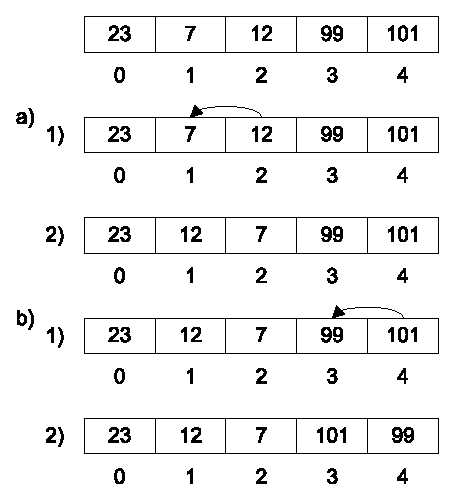
\includegraphics{search_sequential}
\end{center}
\caption{a) Search($12$), b) Search($101$)} \label{fig:search_seq}
\end{figure}

% Copyright (C) Data Structures and Algorithms Team.
\chapter{Sets}

% Copyright (C) Data Structures and Algorithms Team.
\chapter{Strings}
Strings have their own chapter in this text purely because string operations and transformations are incredibly frequent within programs. The algorithms presented are based on problems the authors have come across previously, or were formulated to satisfy curiosity.

\section{Reversing the order of words in a sentence}

\begin{tabbing}
1) \textbf{alg}\= \textbf{orithm} ReverseWords($value$) \\
2) \> \textbf{Pre:}~~ $value~!= \emptyset$, $sb$ is a string buffer \\
3) \> \textbf{Post:}~ the words in $value$ have been reversed \\
4) \> $last \leftarrow value$.Length $-~1$ \\
5) \> $start \leftarrow last$ \\
6) \> \textbf{whi}\= \textbf{le} $last \geq 0$ \\
7) \> \> // skip whitespace \\
8) \> \> \textbf{whi}\= \textbf{le} $start \geq 0$ \textbf{and} $value$[$start$] = whitespace \\
9) \> \> \> $start \leftarrow start - 1$ \\
10)\> \> \textbf{end while} \\
11)\> \> $last \leftarrow start$ \\
12)\> \> // march down to the index before the beginning of the word \\
13)\> \> \textbf{while} $start \geq 0$ \textbf{and} $start~!=$ whitespace \\
14)\> \> \> $start \leftarrow start - 1$ \\
15)\> \> \textbf{end while} \\
16)\> \> // append chars from $start + 1$ to $length + 1$ to string buffer sb \\
17)\> \> \textbf{for} $i \leftarrow start + 1$ \textbf{to} $last$ \\
18)\> \> \> $sb$.Append($value$[$i$]) \\
19)\> \> \textbf{end for} \\
20)\> \> // if this isn't the last word in the string add some whitespace after the word in the buffer \\
21)\> \> \textbf{if} $start > 0$ \\ 
22)\> \> \> $sb$.Append(` ') \\
23)\> \> \textbf{end if} \\
24)\> \> $last \leftarrow start - 1$ \\
25)\> \> $start \leftarrow last$ \\
26)\> \textbf{end while} \\
27)\> // check if we have added one too many whitespace to $sb$ \\
28)\> \textbf{if} $sb$[$sb$.Length $- 1$] = whitespace \\
29)\> \> // cut the whitespace \\
30)\> \> $sb$.Length $\leftarrow sb$.Length $- 1$ \\
31)\> \textbf{end if} \\
32)\> \textbf{return} $sb$ \\
33) \textbf{end} ReverseWords \\
\end{tabbing}


\appendix
% Copyright (C) Data Structures and Algorithms Team.
\chapter{Translation Walkthrough}
The conversion from pseudo to an actual imperative language is usually very straight forward, to clarify an example is provided.
In this example we will convert the algorithm in \S\ref{cha:Primality} to the C\# language.

\begin{tabbing}
1) pub\=lic static bool IsPrime(int number) \\
2) \{ \\
3) \> if (\=number $<$ 2) \\
4) \> \{ \\
5) \> \> return false; \\
6) \> \} \\ 
7) \> int innerLoopBound $=$ (int)Math.Floor(Math.Sqrt(number)); \\
8) \> for (int i $=$ 1; i $<$ number; i++) \\
9) \> \{ \\
10) \> \> for\= (int j $=$ 1; j $<=$ innerLoopBound; j++) \\
11) \> \> \{ \\
12) \> \> \> if (\=i $*$ j $==$ number) \\
13) \> \> \> \{ \\
14) \> \> \> \> return false; \\
15) \> \> \> \} \\
16) \> \> \} \\
17) \> \} \\
18) \> return true; \\
19) \} \\
\end{tabbing}

For the most part the conversion is a straight forward process, however you may have to inject various calls to other utility algorithms to ascertain the correct result.

A consideration to take note of is that many algorithms have fairly strict preconditions, of which there may be several - in these scenarios you will need to inject the correct code to handle such situations to preserve the correctness of the algorithm. Most of the preconditions can be suitably handled by throwing the correct exception.

% Copyright (C) Data Structures and Algorithms Team.
\chapter{Symbol Definitions}
Throughout the pseudocode listings you will find several symbols used,  describes the meaning of each of those symbols.

\begin{table}[h]
\caption{Pseudo symbol definitions}
\begin{tabular}[t]{|c|l|}
\hline
\textbf{Symbol} & \textbf{Description} \\
\hline
$\leftarrow$ & Assignment. In most imperative languages this equates to $=$ \\
\hline
$=$ & Equality. Most imperative languages use $==$ to denote a check for equality. \\
\hline
$\leq$ & Less than or equal to. Commonly this is denoted as $<=$ in imperative languages. \\
\hline
$<$ & Less than.* \\
\hline
$\geq$ & Greater than or equal to. Commonly this is denoted as $>=$ in imperative languages. \\
\hline
$>$ & Greater than.* \\
\hline
$!=$ & Inequality. * \\
\hline
$\emptyset$ & Null. \\
\hline
\textbf{and} & Logical and. Commonly \&\& in imperative languages. \\
\hline
\textbf{or} & Logical or. Commonly || in imperative languages. \\ 
\hline
whitespace & Correct token in your language that represents whitespace. \\
\hline
\textbf{yield} & Like \textbf{return} but builds a sequence. \\
\hline
\end{tabular}
\end{table}

* This symbol has a direct translation with the vast majority of imperative counterparts.


\end{document}
